% compile with xelatex
% !TeX program = xelatex

%%%%%%%%%%%%%%%%%%%%%%%%%%%%%%%%%%%%%%%%%%%%%%%%%%%%%%%%%%%%%%%%%
% Compile with:
%
% $ latexmk -xelatex -pvc slides
%%%%%%%%%%%%%%%%%%%%%%%%%%%%%%%%%%%%%%%%%%%%%%%%%%%%%%%%%%%%%%%%%

%%%%%%%%%%%%%%%%%%%%%%%%%%%%%%%%%%%%%%%%%%%%%%%%%%%%%%%%%%%%%%%%%
% This document has the following requirements:
% - Fira Code
%   - see https://github.com/tonsky/FiraCode/wiki/Installing
% - Xelatex
%   - This should be automatically activated by the magic comment above,
%     But VSCode prevents this. Use the following setting to allow the
%     magic comment to work:
%     latex-workshop.latex.build.forceRecipeUsage: false
%     This setting should already be set by the workspace settings
%
% The manual is here:
% https://mirrors.dotsrc.org/ctan/macros/latex/contrib/beamer-contrib/themes/metropolis/doc/metropolistheme.pdf
%
%%%%%%%%%%%%%%%%%%%%%%%%%%%%%%%%%%%%%%%%%%%%%%%%%%%%%%%%%%%%%%%%%

%%%%%%%%%%%%%%%%%%%%%%%%%%%%%%%%%%%%%%%%%%%%%%%%%%%%%%%%%%%%%%%%%
% Trouble shotting:
%
% If you get this error:
%
%   Couldn't open `Fira Mono .cfg'
%   Sorry, but miktex-maketfm did not succeed.
%
% then go to: https://github.com/mozilla/Fira
% and download the repository, and
% install the fonts in the OTF folder.
%
%%%%%%%%%%%%%%%%%%%%%%%%%%%%%%%%%%%%%%%%%%%%%%%%%%%%%%%%%%%%%%%%%
\documentclass[aspectratio=169]{beamer}
\usepackage{amsfonts}
\usepackage{amsmath}
\usepackage{amssymb}
\usepackage{amsthm}
\usepackage{datetime}
\usepackage{flix}
\usepackage{fontspec}
\usepackage{graphicx}
\usepackage{listings}
\usepackage{lstfiracode}
\usepackage{microtype}
\usepackage{multicol}
\usepackage{oubraces}
\usepackage{pgf}
\usepackage{tikz}
\usepackage{xcolor}

\newcommand{\DayOne}{Tuesday}
\newcommand{\DayTwo}{Thursday}

\newcommand{\Highlight}[1]{\colorbox{black!10}{$\displaystyle#1$}}

\newcommand{\remark}[1]{{\color{red} \textbf{$\triangleright$ #1 $\triangleleft$}}}

\let\Code\lstinline

\lstset{language=flix}


\usetheme{metropolis}


\title{Week 3}
\date{\today{} at \currenttime{}}
\author{Magnus Madsen}

\begin{document}

\maketitle

\begin{frame}{Week 3: Outline}
\begin{columns}
\begin{column}{.05\textwidth}
\rotatebox{90}{\large \textbf{\DayOne{}}}
\end{column}
\begin{column}{.95\textwidth}
    \footnotesize
\textbf{Lecture} (45min)  \vspace{-2mm}
\begin{itemize}
    \setlength\itemsep{-0.5em}
    \item Introduction to Prolog
    \item Introduction to Unification
\end{itemize}
\textbf{Exercises} (45min) \vspace{-2mm}
\begin{itemize}
    \item Work on the assignment alone or together in small groups.
\end{itemize}
\end{column}
\end{columns}

\medskip
\medskip
\medskip

\begin{columns}
\color{gray}
\begin{column}{.05\textwidth}
\rotatebox{90}{\large \textbf{\DayTwo{}}}
\end{column}
\begin{column}{.95\textwidth}
\footnotesize
\textbf{Lecture} (45min) \vspace{-2mm}
\begin{itemize}
    \color{gray}
    \setlength\itemsep{-0.5em}
    \item A Larger Example: The Wolf, Goat, and Cabbage Problem
\end{itemize}
\textbf{Exercises} (45min)  \vspace{-2mm}
\begin{itemize}
    \color{gray}
    \item Work on the assignment alone or together in small groups.
\end{itemize}
\end{column}
\end{columns}
\end{frame}

\begin{frame}{Quote of the Day}
``As Will Rogers would have said, \emph{there is no such thing as a free variable.}''

\begin{flushright}
--- Alan Perlis
\end{flushright}
\end{frame}

\begin{frame}{Pull Requests are Welcome}
\begin{columns}
\begin{column}{.50\textwidth}
You can improve the course material!

\begin{itemize}
    \item Exercises are in \texttt{src/weekX.md}
    \item Slides are in \texttt{slides/weekX.tex}
\end{itemize}

\medskip

PRs can be submitted on GitHub:
\begin{center}
\scriptsize
\url{https://github.com/magnus-madsen/advprog/}
\end{center}
\end{column}
\begin{column}{.50\textwidth}
    % Source: https://www.q-files.com/history/ancient-egypt/pyramids-how-they-were-built
    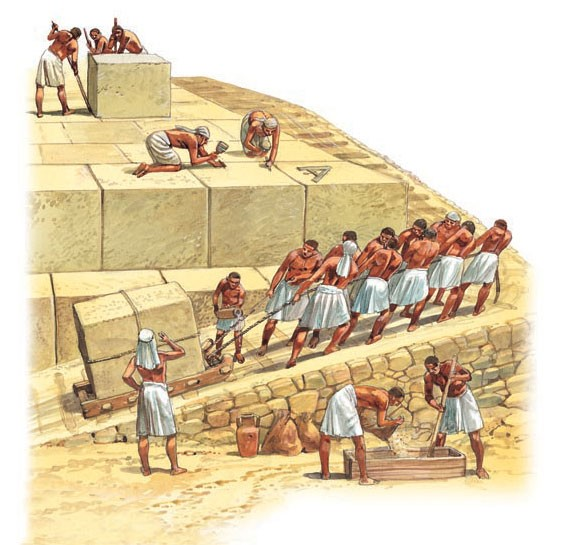
\includegraphics[width=\textwidth]{img/pyramids.jpg}
\end{column}
\end{columns}
\end{frame}


\section{Introduction to Prolog}

\begin{frame}{Prolog}
\Large
Prolog: \emph{Pro}gramming \emph{Log}ic
\end{frame}    

\begin{frame}{From Datalog to Prolog: A Shift in Perspective}
Datalog is based on \emph{bottom-up} tabling:

\begin{itemize}
    \item Datalog has a unique minimal model.
    \item Datalog offers strong guarantees about termination.
    \item Limited expressive power.
\end{itemize}

\pause

Prolog is based on \emph{top-down} search:

\begin{itemize}
    \item Prolog is goal-driven.
    \item Prolog programs are imperative: the order of evaluation matters.
    \item Prolog is Turing-complete -- and hence programs may fail to terminate.
\end{itemize}

\pause

Prolog \emph{is} a logic programming language, but it is like the C of logic languages.
\end{frame}

\begin{frame}{Expressive Power}
% Copied from week2.tex
\centering
\medskip
\medskip
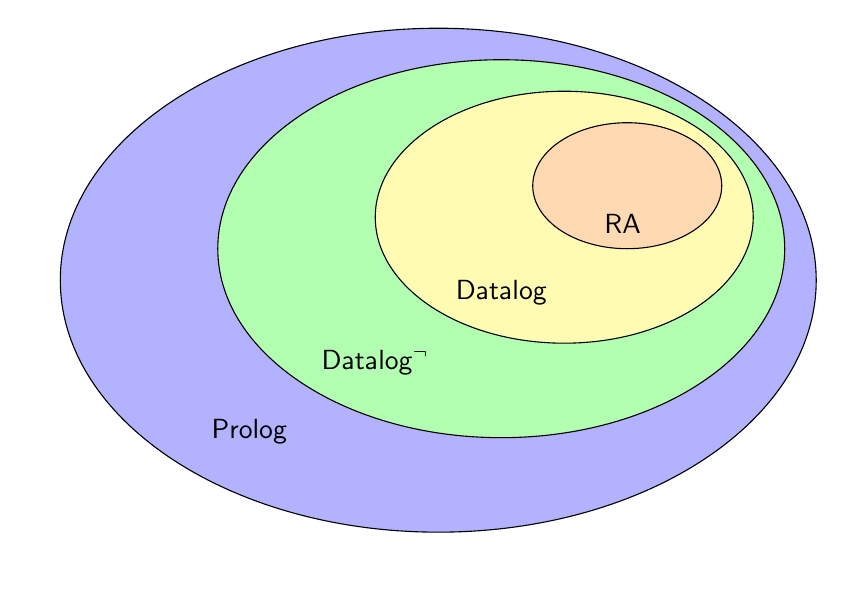
\begin{tikzpicture}[font=\sffamily, scale=0.8]
\foreach \X/\col [count=\N, evaluate=\N as \Y using 5-\N] in {Prolog/blue, Datalog$^\neg$/green, Datalog/yellow, RA /orange}
{\draw[fill=\col!30] (-\Y,-\Y/2) circle ({1.5*\Y} and \Y);
\node[align=center] at (1-2*\Y,-1.1*\Y) {\X}; }
\draw ([xshift=-0.5cm,yshift=-0.5cm] current bounding box.south west);
\end{tikzpicture}
\end{frame}

\begin{frame}[fragile]{Syntax Update}
In Flix the syntax of a rule is:

\begin{lstlisting}[language=flix, xleftmargin=0.5cm]
Path(x, z) :- Edge(x, y), Path(y, z).
\end{lstlisting}

In Prolog the syntax of the same rule is:

\begin{lstlisting}[language=prolog, xleftmargin=0.5cm]
path(X, Z) :- edge(X, Y), path(Y, Z).
\end{lstlisting}

\pause

Moreover, in Prolog lowercase names are constants:

\begin{lstlisting}[language=prolog, xleftmargin=0.5cm]
parent(emma, magnus).
parent(emma, daniela).
\end{lstlisting}

\pause

\textbf{Warning:} You will screw this up. Remember to check your casing. 
\end{frame}

\begin{frame}{Prolog is Query Driven}
To write a Prolog program: 

\begin{itemize}
    \item We state the facts and rules of the domain.
    \item We ask a query (with zero or more free variables).
\end{itemize}

Prolog computes a \textbf{\emph{single}} solution answering \textbf{yes} or \textbf{no}.

\medskip

Here we can see Prolog's roots in expert systems and artificial intelligence.
\end{frame}

\begin{frame}[fragile]{A Few Simple Queries (1/3)}
Given the facts:

\begin{lstlisting}[language=prolog, xleftmargin=0.5cm]
parent(emma, magnus).
parent(emma, daniela).
\end{lstlisting}

\pause

We can ask:

\begin{lstlisting}[language=prolog, xleftmargin=0.5cm]
?- parent(emma, magnus).
yes
\end{lstlisting}

\pause

And we can ask:

\begin{lstlisting}[language=prolog, xleftmargin=0.5cm]
?- parent(emma, augustus).
no
\end{lstlisting}
\end{frame}

\begin{frame}[fragile]{A Few Simple Queries (2/3)}
We can also ask:

\begin{lstlisting}[language=prolog, xleftmargin=0.5cm]
?- parent(emma, X).
X = magnus ? ;
X = daniela ? ;
no
\end{lstlisting}

We use the semicolon \textbf{;} to prompt Prolog for additional solutions.

Prolog says \textbf{no} at the end because there are no more solutions!
\end{frame}

\begin{frame}[fragile]{A Few Simple Queries (3/3)}
In Prolog \Code{parent} is a relation, not a function, so we can also ask:

\begin{lstlisting}[language=prolog, xleftmargin=0.5cm]
?- parent(X, magnus).
X = emma ? ;
no
\end{lstlisting}

Note that we are asking for ``an input'' that matches ``an output''.

\pause

\textbf{Question}: What is the answer to the query \Code{parent(X, Y)}?
\end{frame}

\begin{frame}[fragile]{Recursion in Prolog (1/2)}
Prolog supports recursion:

\begin{lstlisting}[language=prolog, xleftmargin=0.5cm]
edge(a, b).
edge(b, c).

path(X, Y) :- edge(X, Y).
path(X, Z) :- edge(X, Y), path(Y, Z).
\end{lstlisting}

\pause

And we can ask:

\begin{lstlisting}[language=prolog, xleftmargin=0.5cm]
?- path(a, c).
yes

?- path(a, X).
X = b ? ;
X = c ? ;
no
\end{lstlisting}
\end{frame}

\begin{frame}[fragile]{Recursion in Prolog (2/2)}
But we have to be careful. If we change the program to:

\begin{lstlisting}[language=prolog, xleftmargin=0.5cm]
path(X, Z) :- path(Y, Z), edge(X, Y).
path(X, Y) :- edge(X, Y).
\end{lstlisting}

\pause

And ask:

\begin{lstlisting}[language=prolog, xleftmargin=0.5cm]
?- path(a, c).
\end{lstlisting}

\pause

The program loops! But why?

\pause

\textbf{Answer:} Prolog uses top-to-bottom, left-to-right evaluation.
\end{frame}

\begin{frame}{Constructors in Prolog (1/2)}
Prolog supports constructors:

\begin{itemize}
    \item Allows us to construct compound value (lists, trees, etc).
    \item Allows us to construct infinite values (oops.)
\end{itemize}

Like in functional programming, we use constructors to build data structures.
\end{frame}

\begin{frame}[fragile]{Constructors in Prolog (2/2)}
We can write:

\begin{lstlisting}[language=prolog, xleftmargin=0.5cm]
networth(person(steve, carrel),   80). % in millions USD
networth(person(steve, jobs),    250). % in millions USD
networth(person(jeff, bezos), 186000). % in millions USD
\end{lstlisting}

\pause

And then we can ask:

\begin{lstlisting}[language=prolog, xleftmargin=0.5cm]
?- networth(X, 80).
X = person(steve,carrel)
\end{lstlisting}

\pause

We can also ask:

\begin{lstlisting}[language=prolog, xleftmargin=0.5cm]
?- networth(person(steve, X), Y).
X = carrel, Y =  80 ? ;
X = jobs,   Y = 250 ? ;
\end{lstlisting}
\end{frame}

\begin{frame}[fragile]{Lists in Prolog (1/2)}
We can use constructors to encode lists:

\begin{lstlisting}[language=prolog, xleftmargin=0.5cm]
len(nil, 0).
len(cons(_, Xs), R) :- len(Xs, N), R is N + 1.
\end{lstlisting}

\pause

And then we can ask:

\begin{lstlisting}[language=prolog, xleftmargin=0.5cm]
len(cons(1, cons(2, cons(3, nil))), N).
N = 3 ? ;
\end{lstlisting}

\pause

\textbf{Note:} Please use the built-in lists: \Code{[]} and \Code{[Head|Tail]}
in real programs. 
\end{frame}

\begin{frame}[fragile]{Lists in Prolog (2/2)}
We can also write:

\begin{lstlisting}[language=prolog, xleftmargin=0.5cm]
appnd(nil, Ys, Ys).
appnd(cons(X, Xss), Ys, cons(X, Rs)) :- appnd(Xss, Ys, Rs).
\end{lstlisting}

\pause

And then we can ask:

\begin{lstlisting}[language=prolog, xleftmargin=0.5cm]
?- appnd(cons(1, cons(2, nil)), cons(3, cons(4, nil)), R).
R = cons(1,cons(2,cons(3,cons(4,nil)))) ? ;
\end{lstlisting}
\end{frame}

\begin{frame}[fragile]{Arithmetic in Prolog}
We wrote:

\begin{lstlisting}[language=prolog, xleftmargin=0.5cm]
R is N + 1.
\end{lstlisting}

because wanted to force Prolog to evaluate \Code{R} to \Code{N + 1}. 

Note that:

\begin{lstlisting}[language=prolog, xleftmargin=0.5cm]
?- 1 + 2 = 3.   no
?- 3 is 1 + 2.  yes
\end{lstlisting}

\pause

But

\begin{lstlisting}[language=prolog, xleftmargin=0.5cm]
?- 1 + 2 is 3.  no
\end{lstlisting}

The \Code{is} operator forces evaluation \emph{on the right-hand side}.

\end{frame}

\begin{frame}[fragile]{Prolog is Dynamically Typed (1/2)}
Prolog is dynamically typed, so if we write:

\begin{lstlisting}[language=prolog, xleftmargin=0.5cm]
appnd(apple, cons(1, nil), R).
\end{lstlisting}

Prolog just tells us \textbf{no}. This maybe okay.

\pause

But it can also get weird:

\begin{lstlisting}[language=prolog, xleftmargin=0.5cm]
?- appnd(nil, apple, R).
R = apple ? ;
\end{lstlisting}

Here \Code{R} is not a list! Oops!
\end{frame}
    
\begin{frame}[fragile]{Prolog is Dynamically Typed (2/2)}
Like in Scheme, we can add dynamic type checks. We define the list ``type'':

\begin{lstlisting}[language=prolog, xleftmargin=0.5cm]
is_list(nil).
is_list(cons(_, Xs)) :- is_list(Xs).
\end{lstlisting}

\pause

And then we update our implementation of \Code{appnd}:

\begin{lstlisting}[language=prolog, xleftmargin=0.5cm]
appnd(nil, Ys, Ys) :- is_list(Ys).
appnd(cons(X, Xss), Ys, cons(X, Rs)) :- 
    appnd(Xss, Ys, Rs), is_list(Xss), is_list(Ys), is_list(Rs).
\end{lstlisting}

Now our silly query \Code{?- appnd(nil, apple, R)} returns \textbf{no}.
\end{frame}

\begin{frame}{Prolog Grammar}
The core Prolog grammar is almost equivalent to the Datalog grammar:
{
\large
\begin{align*}
p \in \textsl{Program}      &= c_1 \cdots c_n \\
c \in \textsl{Constraint}   &= A_0 \Leftarrow B_1, \cdots, B_n. \\ 
A \in \textsl{HeadAtom}     &= p(t_1, \cdots, t_n) \\
B \in \textsl{BodyAtom}     &= p(t_1, \cdots, t_n) \mid \Highlight{\textbackslash+} \, p(t_1, \cdots, t_n) \\
t \in \textsl{Term}         &= k \mid x \mid \Highlight{c (t_1, \cdots, t_n)} \\
\\
p \in \textsl{Predicates}   & = \text{is a finite set of predicate symbols.} \\
x \in \textsl{Variables}    & = \text{is a finite set of variable symbols.} \\
\Highlight{c \in \textsl{Constructors}} & = \Highlight{\text{is a finite set of constructors.}} \\
k \in \textsl{Constants}    & = \text{is a finite set of constants.}
\end{align*}
}
\end{frame}

\section{Unification}

\begin{frame}[fragile]{Matching a Goal to a Rule}
Assume we have a Prolog program with the facts and rules:

\begin{lstlisting}[language=prolog, xleftmargin=0.5cm]
len([], 0).
len([_Head|Tail], R) :- len(Tail, N), R is N + 1.
\end{lstlisting}

\pause 

And we ask Prolog the query:

\begin{lstlisting}[language=prolog, xleftmargin=0.5cm]
? len([1, 2], X).
\end{lstlisting}

which is really: 

\begin{lstlisting}[language=prolog, xleftmargin=0.5cm]
? len([1 | [2 | []]], X).
\end{lstlisting}

\textbf{Question:} How does Prolog know which rule to evaluate?

\textbf{Question:} And what should be the values of the variables in the rule?

\pause 

\textbf{Answer:} Prolog uses \textbf{\emph{unification}} to match the goal with
the head atom.
\end{frame}   

\begin{frame}{What is Unification (1/2)}
A \textbf{\emph{substitution}} is a map from variables to terms.

\pause

For example, we can have the substitution:
\[
    s = \{ X \mapsto 21, Y \mapsto [1, 2, 3] \} 
\]

\pause

We can apply a substitution to a term. For example, 

if $t = node(X, X, Y)$ then 
\[
    s(t) = node(21, 21, [1, 2, 3])
\]
\end{frame}  

\begin{frame}{What is Unification? (1/2)}
A \textbf{\emph{substitution}} is a map from variables to terms.

\pause

For example, we can have the substitution:
\[
    s = \{ X \mapsto 21, Y \mapsto [1, 2, 3, W] \} 
\]

\pause

We can apply a substitution to a term. For example: 

If $t = node(X, X, Y)$ then 
\[
    s(t) = node(21, 21, [1, 2, 3, W])
\]
\end{frame}  

\begin{frame}{What is Unification? (2/2)}
\textbf{Unification}: Given two terms $t_1$ and $t_2$, find a substitution $s$
such that:
%
\[
    s(t_1) = s(t_2)
\]
%
The substitution, when applied to both terms, makes them \emph{syntactically} equal. 
%
\begin{itemize}
    \item We call such a substitution a \emph{unifier}. It may not always exist.
    \item But if there is a unifier then there is a \emph{most-general unifier} (MGU).
\end{itemize}

\pause

\textbf{Sidenote:} A cool idea is when $=$ is replaced by $\equiv$ leading to
\textbf{E-unification}, i.e. unification modulo some equational theory. 
\end{frame}  

\begin{frame}[fragile]{A Unification Algorithm (in Flix) (1/6)}
We define the language of terms:

\begin{lstlisting}[language=flix, xleftmargin=0.5cm]
enum Term {
    case Var(String),
    case Cst(Int32),
    case Pair(Term, Term)
}
\end{lstlisting}

A real term language, like the one used in Prolog, is richer.

However, the above term language is sufficient to illustrate the major points. 
\end{frame}

\begin{frame}[fragile]{A Unification Algorithm (in Flix) (2/6)}
We define a substitution as:

\begin{lstlisting}[language=flix, xleftmargin=0.5cm]
type alias Subst = Map[String, Term]
\end{lstlisting}

\pause

And we define a function that applies a substitution to a term:

\begin{lstlisting}[language=flix, xleftmargin=0.5cm]
def applySubst(s: Subst, t: Term): Term = match t {
    case Term.Var(x)        => Map.getWithDefault(x, t, s)
    case Term.Cst(c)        => Term.Cst(c)
    case Term.Pair(t1, t2)  => 
        Term.Pair(applySubst(s, t1), applySubst(s, t2))
}
\end{lstlisting}
\end{frame}

\begin{frame}[fragile]{A Unification Algorithm (in Flix) (3/6)}
Given two substitutions $s_1$ and $s_2$, we define a function to compose them.

The new substitution should morally have the effect of applying $s_1$ to the
term and then applying $s_2$ to that, i.e. we want:
%
\[
    \text{compose}(s_1, s_2)(t) = s_2(s_1(t))
\]

\textbf{Implementation:} Left as an exercise for the reader.

\textbf{Remark:} Most bugs happen when implementing compose. 
\end{frame}

\begin{frame}[fragile]{A Unification Algorithm (in Flix) (4/6)}
We can now write a function to unify two terms:

\begin{lstlisting}[language=flix, xleftmargin=0.5cm]
def unify(t1: Term, t2: Term): Subst = match (t1, t2) {
    case (Term.Cst(c1), Term.Cst(c2)) if c1 == c2 => Map.empty()
    case (Term.Var(x), _) => Map.singleton(x, t2)
    case (_, Term.Var(y)) => Map.singleton(y, t1)
    case (Term.Pair(t11, t12), Term.Pair(t21, t22)) => 
        let s1 = unify(t11, t21);
        let s2 = unify(applySubst(s1, t12), applySubst(s1, t22));
        compose(s1, s2)
    case _ => unsafe throw new Exception("Unification failed")
}
\end{lstlisting}

\pause

\textbf{Question:} Why apply \Code{s1} to \Code{t12} and \Code{t22} before the
recursive call to \Code{unify}?
\end{frame}  

\begin{frame}[fragile]{A Unification Algorithm (in Flix) (5/6)}
Lets try it out: 

\begin{lstlisting}[language=flix, xleftmargin=0.5cm]
unify(Cst(123), Var("x")) 
    => Map#{x => Cst(123)}
\end{lstlisting}

\pause 

\begin{lstlisting}[language=flix, xleftmargin=0.5cm]
unify(Pair(Var("x"), Var("x")), Pair(Cst(123), Var("y"))) 
    => Map#{x => Cst(123), y => Cst(123)}
\end{lstlisting}

\pause 

What about:

\begin{lstlisting}[language=flix, xleftmargin=0.5cm]
unify(Var("x"), Pair(Cst(123), Var("x")))
    => Map#{x => Pair(Cst(123), Var(x))}
\end{lstlisting}

\pause 

\textbf{Ooos!} This is incorrect. What's the problem?

\end{frame}

\begin{frame}[fragile]{A Unification Algorithm (in Flix) (6/6)}
We modify the two cases for variables as follows: 

\begin{lstlisting}[language=flix, xleftmargin=0.5cm]
case (Term.Var(x), t2) => 
    if (Set.memberOf(x, freeVars(t2)))
        unsafe throw new Exception("Occurs Check") 
    else 
        Map.singleton(x, t2)

// The other case is symmetric.
\end{lstlisting}

Here the \Code{freeVars} function is defined in the obvious way.

The \textbf{occurs check} ensures that we do not construct substitutions where a
variable occurs recursively within the term it is unified with. 

\pause

\textbf{Note:} The occurs check is expensive, so some Prolog implementations omit it.
\end{frame}  

\begin{frame}[fragile]{Matching a Goal to a Rule -- Continued (1/2)}
Recall that we had: 

\begin{lstlisting}[language=prolog, xleftmargin=0.5cm]
len([], 0).
len([_Head|Tail], R) :- len(Tail, N), R is N + 1.
\end{lstlisting}

\pause

And we ask: 

\begin{lstlisting}[language=prolog, xleftmargin=0.5cm]
? len([1 | [2 | []]], X).
\end{lstlisting}

\pause

Prolog uses unification to the determine that:

\begin{enumerate}
    \item We cannot unify $[]$ with $[1 | [2 | []]]$ so the first rule (fact) is
    not applicable. \pause 
    \item We \emph{can} unify $[\_Head|Tail]$ with $[1 | [2 | []]]$ using the
    substitution $\{ \text{\_Head} \mapsto 1, \text{Tail} \mapsto [2 | []] \}$. \pause
    \item We then apply the substitution to the rule body to obtain the new
    goals: $\text{len}([2 | []], R)$ and $R \text{ is } X + 1$, and recurse.
\end{enumerate}
\end{frame}

\begin{frame}[fragile]{Matching a Goal to a Rule -- Continued (2/2)}
To recap:

\begin{itemize}
    \pause \item Prolog searches for a fact or rule \emph{from top to bottom} of the
    file where the current goal unifies with the head atom.
    \pause \item If a match is found, Prolog applies the found substition to the rule
    body which now become the sub-goals of the query. 
    \pause \item The sub-goals are evaluated from left to right.
    \pause \item A goal is satisfied once we reach a fact.
\end{itemize}

\pause Hence: Be careful about evaluation order. It matters!
\end{frame}

\begin{frame}[fragile]{Print Debugging is Back! (1/2)}
If we write: 

\begin{lstlisting}[language=prolog, xleftmargin=0.5cm]
edge(1, 2).
edge(2, 3).
path(X, Y) :- edge(X, Y), write('rule1\n').
path(X, Z) :- edge(X, Y), path(Y, Z), write('rule2\n').
\end{lstlisting}

\pause And ask:

\begin{lstlisting}[language=prolog, xleftmargin=0.5cm]
-? path(1, 3).
\end{lstlisting}

\pause Prolog prints:

\begin{lstlisting}[language=prolog, xleftmargin=0.5cm]
rule1
rule2
yes
\end{lstlisting}
\end{frame}

\begin{frame}[fragile]{Print Debugging is Back! (2/2)}
We can explore Prolog's evaluation order by writing:

\begin{lstlisting}[language=prolog, xleftmargin=0.5cm]
path(X, Z) :- write('A'), edge(X, Y), write('B'), path(Y, Z), write('C').
\end{lstlisting}

And asking:

\begin{lstlisting}[language=prolog, xleftmargin=0.5cm]
-? path(1, 3).
\end{lstlisting}

\pause \textbf{Question:} What does this print?
\end{frame}

\begin{frame}{Prolog Extensions}
Prolog comes with several extensions:

\begin{itemize}
    \item Cuts (a mechanism to control backtracking)
    \item Higher-order predicates (e.g. \Code{findall})
    \item Reflection (e.g. \Code{clause})
    \item Tabling (ala Datalog)
\end{itemize}

You will most likely need some of these for any serious Prolog programming. 
\end{frame}

\section{A Larger Example}

\begin{frame}{The Wolf, Goat, and Cabbage Problem (1/2)}
\begin{center}
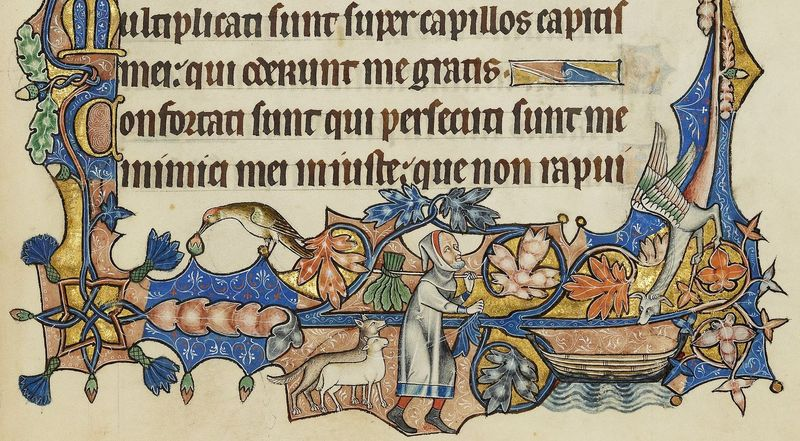
\includegraphics[width=0.75\textwidth]{img/river-problem.jpg}
\end{center}
\begin{small}
``The wolf, goat, and cabbage problem is a river crossing puzzle. It dates back
to at least the 9th century and has entered the folklore of several cultures.'' -- \textsl{Wikipedia}
\end{small}
\end{frame}

\begin{frame}{The Wolf, Goat, and Cabbage Problem (2/2)}
Via Wikipedia:

\bigskip

\begin{quote}
``A \textbf{farmer} with \textbf{a wolf}, \textbf{a goat}, and \textbf{a
cabbage} must cross a river by boat. The boat can carry only the farmer and a
single item. If left unattended together, the wolf would eat the goat, or the
goat would eat the cabbage. How can they cross the river without anything being
eaten?''
\end{quote}

\bigskip

We can solve this problem with Prolog. 

\pause

\textbf{Question:} But can you solve it with your brain? (and some paper...)
\end{frame}

\begin{frame}[fragile]{Wolf, Goat, and Cabbage in Prolog (1/8)}
We consider the river to have two sides: the \textbf{west bank} (\Code{w}) and
\textbf{east bank} (\Code{e}).

Initially, everyone will be on the west bank.

We can then define that one can travel from west to east and east to west:

\begin{lstlisting}[language=prolog, xleftmargin=0.5cm]
travel(w, e). 
travel(e, w).
\end{lstlisting}

We further assume we have three constants: \Code{farmer}, \Code{wolf},
\Code{goat}, \Code{cabbage}.
\end{frame}

\begin{frame}[fragile]{Wolf, Goat, and Cabbage in Prolog (2/8)}
We define a configuration of the problem as a 4-tuple (using a list):
%
We order the travelers as: \Code{farmer}, \Code{wolf}, \Code{goat},
\Code{cabbage}. Now:
%
\begin{itemize}
    \item The list: \Code{[w, w, w, w]} means that everyone is on the west bank.
    \item The list: \Code{[e, e, e, e]} means that everyone is on the east bank.
    \item The list: \Code{[e, e, e, w]} means that the farmer, wolf, and goat is
    on the east bank whereas the cabbage is on the west bank --- which is okay.
    \item The list: \Code{[e, w, w, e]} means that the farmer and cabbage is on
    the east bank whereas the wolf and the goat is on the east bank --- which is
    NOT OKAY!
\end{itemize}
\end{frame}
    
\begin{frame}[fragile]{Wolf, Goat, and Cabbage in Prolog (3/8)}
We now define a ternary relation: \texttt{move(state1, moved, state2)}:

If the farmer and wolf are on the west bank then they can travel to the east bank. 

The goat and cabbage stay where they are. 

We can capture this with the fact:

\begin{lstlisting}[language=prolog, xleftmargin=0.5cm]
move([w, w, G, C], wolf, [e, e, G, C]).
\end{lstlisting}

\pause

They can also travel back, so we need:

\begin{lstlisting}[language=prolog, xleftmargin=0.5cm]
move([e, e, G, C], wolf, [w, w, G, C]).
\end{lstlisting}

\pause

This is a bit tedious, so let us make use of \Code{travel}:

\begin{lstlisting}[language=prolog, xleftmargin=0.5cm]
move([X, X, G, C], wolf, [Y, Y, G, C]) :- travel(X, Y).
\end{lstlisting}
\end{frame}

\begin{frame}[fragile]{Wolf, Goat, and Cabbage in Prolog (4/8)}
We have:

\begin{lstlisting}[language=prolog, xleftmargin=0.5cm]
move([X, X, G, C], wolf, [Y, Y, G, C]) :- travel(X, Y).
\end{lstlisting}

\pause

and we need three more rules:

\begin{lstlisting}[language=prolog, xleftmargin=0.5cm]
move([X, W, X, C], goat,    [Y, W, Y, C]) :- travel(X, Y).
move([X, W, G, X], cabbage, [Y, W, G, Y]) :- travel(X, Y).
move([X, W, G, C], nothing, [Y, W, G, C]) :- travel(X, Y).    
\end{lstlisting}

\pause

\textbf{Question:} Why do we need the last rule?
\end{frame}

\begin{frame}[fragile]{Wolf, Goat, and Cabbage in Prolog (5/8)}

\textbf{Recall:} We want to ensure that the (a) wolf does not eat the goat, and
(b) the goat does not eat the cabbage.

We define the states that are safe. There are two cases: 

(1) The goat is on the same bank as the farmer:

\begin{lstlisting}[language=prolog, xleftmargin=0.5cm]
safe([X, _, X, _]).  // Recall: farmer, wolf, goat, cabbage
\end{lstlisting}

(2) Or the wolf and cabbage are on the same bank as the farmer:

\begin{lstlisting}[language=prolog, xleftmargin=0.5cm]
safe([X, X, _, X]).
\end{lstlisting}

\pause 

\textbf{Question:} Are (1) and (2) equivalent to (a) and (b)?

\end{frame}

\begin{frame}[fragile]{Wolf, Goat, and Cabbage in Prolog (6/8)}
We can now define a solution: A solution is a pair of a state and a list of
moves that brings everyone safely to the east bank.

\pause

If everyone is already on the east bank there is nothing to be done:

\begin{lstlisting}[language=prolog, xleftmargin=0.5cm]
solution([e, e, e, e], []).
\end{lstlisting}

\pause 

We can move to a new state provided that it is (i) safe and (ii) solvable:

\begin{lstlisting}[language=prolog, xleftmargin=0.5cm]
solution(State, [FirstMove | OtherMoves]) :- 
    move(State, FirstMove, NextState), 
    safe(NextState), 
    solution(NextState, OtherMoves).
\end{lstlisting}
\end{frame}

\begin{frame}[fragile]{Wolf, Goat, and Cabbage in Prolog (7/8)}
We can now ask Prolog to compute a solution:

\begin{lstlisting}[language=prolog, xleftmargin=0.5cm]
? solution([w, w, w, w], X).
\end{lstlisting}

\pause 

And then we wait ...

\pause 

And then we wait some more ...

\pause 

And, hey, what's happening?

\pause 

\textbf{Problem:} We have infinitely many moves leading to no solution. The
farmer is just going back and forth, forever. 
\end{frame}

\begin{frame}[fragile]{Wolf, Goat, and Cabbage in Prolog (8/8)}
\textbf{Solution:} We (indirectly) bound the recursion depth.

\pause

How? We fix the length of the list with moves:

\begin{lstlisting}[language=prolog, xleftmargin=0.5cm]
? length(X, 7), solution([w, w, w, w], X).
\end{lstlisting}

\pause

Prolog now answers:

\begin{lstlisting}[language=prolog, xleftmargin=0.5cm]
X = [goat, nothing, wolf, goat, cabbage, nothing, goat]
\end{lstlisting}

\pause

\textbf{Question:} Why did I choose 7? How did I know what number to choose?

\pause

\bigskip 
\scriptsize
% https://danielschlegel.org/wp/teaching/prolog-farmer-goat-wolf-cabbage/
Example inspired by UCSD: {\tiny \url{https://cseweb.ucsd.edu/classes/fa09/cse130/misc/prolog/goat_etc.html}}
\end{frame}

\section{Getting Started with Prolog}

\begin{frame}{Prolog Dialects and Implementations}
As with Datalog there are many Prolog dialects and implementations.

The most popular and battle-tested Prolog implementations are:

\begin{itemize}
    \item \textbf{Ciao Prolog} is an open-source research project from UPM and IMDEA 
        \linebreak {\small \url{https://ciao-lang.org/}}
    \item \textbf{Gnu Prolog} is an open-source Prolog implementation 
        \linebreak {\small \url{http://www.gprolog.org/}}
    \item \textbf{SWI Prolog} is an open-source Prolog implementation 
        \linebreak {\small \url{https://www.swi-prolog.org/}}
    \item \textbf{XSB Prolog} is a commercial Prolog implementation with tabling
        \linebreak {\small \url{https://xsb.com/xsb-prolog/}}
\end{itemize}
\end{frame}

\begin{frame}{Ciao Prolog}
I recommend that you use \textbf{Ciao Prolog} (with SWI Prolog as backup)
\begin{columns}
\begin{column}{.7\textwidth}
\begin{itemize}
    \item Ciao has been developed for more than 40 years.
    \item Ciao is large research project with many cool ideas. 
    \item Runs in the browser via WebAssembly: \linebreak {\small \url{https://ciao-lang.org/playground/}}
\end{itemize}
\end{column}
\begin{column}{.3\textwidth}
    \centering
    
\includegraphics[width=0.8\columnwidth]{img/ciao-logo.png}
\end{column}
\end{columns}
\end{frame}

\begin{frame}
\begin{tikzpicture}[remember picture,overlay]
    \node[at=(current page.center)] {
        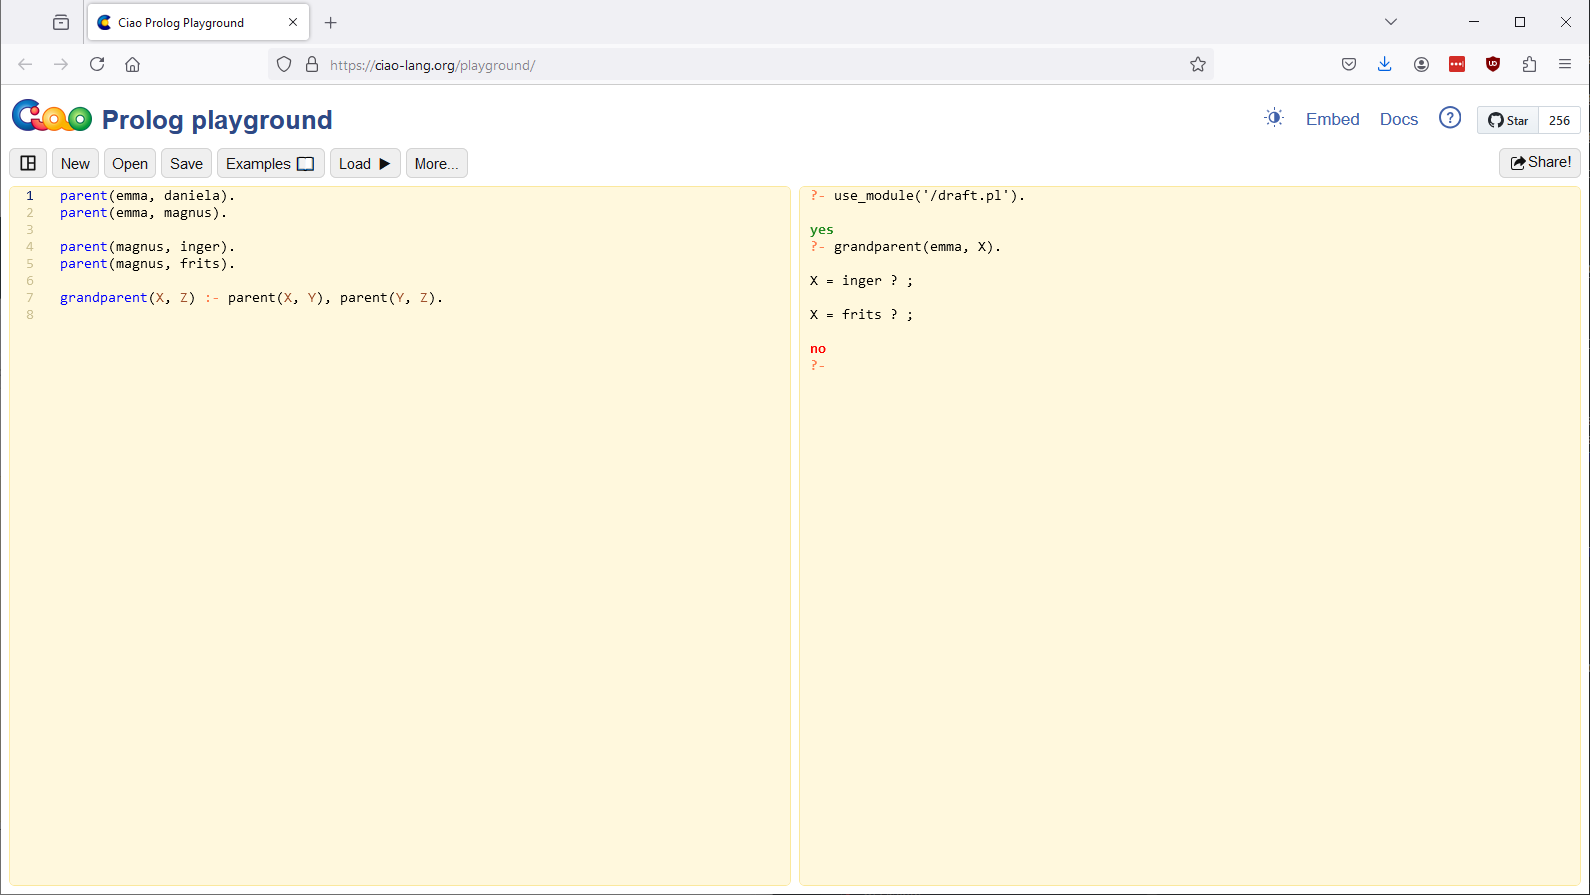
\includegraphics[keepaspectratio,
                        width=\paperwidth,
                        height=\paperheight]{img/ciao-playground.png}
    };
\end{tikzpicture}
\end{frame}

\begin{frame}{Ciao Playground}
Your first task:

\Large
Run the Wolf, Goat, and Cabbage program on the playground.

\bigskip

\centering
{\Large \url{https://ciao-lang.org/playground/}}
\end{frame}

\begin{frame}{Summary}
\textbf{Prolog} is a \textbf{goal-driven} logic programming language:
%
\begin{itemize}
    \item Datalog is for tabling. Prolog is for search. 
\end{itemize}

\pause 

Prolog is Turing-complete. We get the good and the bad: 
%
\begin{itemize}
    \item We can express what we want, but programs may fail to terminate.
\end{itemize}

\pause 

Prolog is less declarative than Datalog: evaluation order matters.

\pause 

Prolog supports compound data types (lists, trees, ...).
\end{frame}
    
    
\begin{frame}[standout]
% blank
\end{frame}

\end{document}
